\documentclass[1p]{elsarticle_modified}
%\bibliographystyle{elsarticle-num}

%\usepackage[colorlinks]{hyperref}
%\usepackage{abbrmath_seonhwa} %\Abb, \Ascr, \Acal ,\Abf, \Afrak
\usepackage{amsfonts}
\usepackage{amssymb}
\usepackage{amsmath}
\usepackage{amsthm}
\usepackage{scalefnt}
\usepackage{amsbsy}
\usepackage{kotex}
\usepackage{caption}
\usepackage{subfig}
\usepackage{color}
\usepackage{graphicx}
\usepackage{xcolor} %% white, black, red, green, blue, cyan, magenta, yellow
\usepackage{float}
\usepackage{setspace}
\usepackage{hyperref}

\usepackage{tikz}
\usetikzlibrary{arrows}

\usepackage{multirow}
\usepackage{array} % fixed length table
\usepackage{hhline}

%%%%%%%%%%%%%%%%%%%%%
\makeatletter
\renewcommand*\env@matrix[1][\arraystretch]{%
	\edef\arraystretch{#1}%
	\hskip -\arraycolsep
	\let\@ifnextchar\new@ifnextchar
	\array{*\c@MaxMatrixCols c}}
\makeatother %https://tex.stackexchange.com/questions/14071/how-can-i-increase-the-line-spacing-in-a-matrix
%%%%%%%%%%%%%%%

\usepackage[normalem]{ulem}

\newcommand{\msout}[1]{\ifmmode\text{\sout{\ensuremath{#1}}}\else\sout{#1}\fi}
%SOURCE: \msout is \stkout macro in https://tex.stackexchange.com/questions/20609/strikeout-in-math-mode

\newcommand{\cancel}[1]{
	\ifmmode
	{\color{red}\msout{#1}}
	\else
	{\color{red}\sout{#1}}
	\fi
}

\newcommand{\add}[1]{
	{\color{blue}\uwave{#1}}
}

\newcommand{\replace}[2]{
	\ifmmode
	{\color{red}\msout{#1}}{\color{blue}\uwave{#2}}
	\else
	{\color{red}\sout{#1}}{\color{blue}\uwave{#2}}
	\fi
}

\newcommand{\Sol}{\mathcal{S}} %segment
\newcommand{\D}{D} %diagram
\newcommand{\A}{\mathcal{A}} %arc


%%%%%%%%%%%%%%%%%%%%%%%%%%%%%5 test

\def\sl{\operatorname{\textup{SL}}(2,\Cbb)}
\def\psl{\operatorname{\textup{PSL}}(2,\Cbb)}
\def\quan{\mkern 1mu \triangleright \mkern 1mu}

\theoremstyle{definition}
\newtheorem{thm}{Theorem}[section]
\newtheorem{prop}[thm]{Proposition}
\newtheorem{lem}[thm]{Lemma}
\newtheorem{ques}[thm]{Question}
\newtheorem{cor}[thm]{Corollary}
\newtheorem{defn}[thm]{Definition}
\newtheorem{exam}[thm]{Example}
\newtheorem{rmk}[thm]{Remark}
\newtheorem{alg}[thm]{Algorithm}

\newcommand{\I}{\sqrt{-1}}
\begin{document}

%\begin{frontmatter}
%
%\title{Boundary parabolic representations of knots up to 8 crossings}
%
%%% Group authors per affiliation:
%\author{Yunhi Cho} 
%\address{Department of Mathematics, University of Seoul, Seoul, Korea}
%\ead{yhcho@uos.ac.kr}
%
%
%\author{Seonhwa Kim} %\fnref{s_kim}}
%\address{Center for Geometry and Physics, Institute for Basic Science, Pohang, 37673, Korea}
%\ead{ryeona17@ibs.re.kr}
%
%\author{Hyuk Kim}
%\address{Department of Mathematical Sciences, Seoul National University, Seoul 08826, Korea}
%\ead{hyukkim@snu.ac.kr}
%
%\author{Seokbeom Yoon}
%\address{Department of Mathematical Sciences, Seoul National University, Seoul, 08826,  Korea}
%\ead{sbyoon15@snu.ac.kr}
%
%\begin{abstract}
%We find all boundary parabolic representation of knots up to 8 crossings.
%
%\end{abstract}
%\begin{keyword}
%    \MSC[2010] 57M25 
%\end{keyword}
%
%\end{frontmatter}

%\linenumbers
%\tableofcontents
%
\newcommand\colored[1]{\textcolor{white}{\rule[-0.35ex]{0.8em}{1.4ex}}\kern-0.8em\color{red} #1}%
%\newcommand\colored[1]{\textcolor{white}{ #1}\kern-2.17ex	\textcolor{white}{ #1}\kern-1.81ex	\textcolor{white}{ #1}\kern-2.15ex\color{red}#1	}

{\Large $\underline{11n_{92}~(K11n_{92})}$}

\setlength{\tabcolsep}{10pt}
\renewcommand{\arraystretch}{1.6}
\vspace{1cm}\begin{tabular}{m{100pt}>{\centering\arraybackslash}m{274pt}}
\multirow{5}{120pt}{
	\centering
	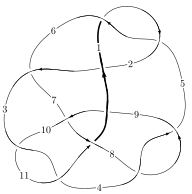
\includegraphics[width=112pt]{../../../GIT/diagram.site/Diagrams/png/708_11n_92.png}\\
\ \ \ A knot diagram\footnotemark}&
\allowdisplaybreaks
\textbf{Linearized knot diagam} \\
\cline{2-2}
 &
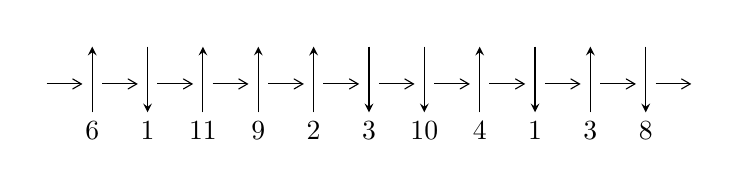
\begin{tikzpicture}[x=20pt, y=17pt]
	% nodes
	\node (C0) at (0, 0) {};
	\node (C1) at (1, 0) {};
	\node (C1U) at (1, +1) {};
	\node (C1D) at (1, -1) {6};

	\node (C2) at (2, 0) {};
	\node (C2U) at (2, +1) {};
	\node (C2D) at (2, -1) {1};

	\node (C3) at (3, 0) {};
	\node (C3U) at (3, +1) {};
	\node (C3D) at (3, -1) {11};

	\node (C4) at (4, 0) {};
	\node (C4U) at (4, +1) {};
	\node (C4D) at (4, -1) {9};

	\node (C5) at (5, 0) {};
	\node (C5U) at (5, +1) {};
	\node (C5D) at (5, -1) {2};

	\node (C6) at (6, 0) {};
	\node (C6U) at (6, +1) {};
	\node (C6D) at (6, -1) {3};

	\node (C7) at (7, 0) {};
	\node (C7U) at (7, +1) {};
	\node (C7D) at (7, -1) {10};

	\node (C8) at (8, 0) {};
	\node (C8U) at (8, +1) {};
	\node (C8D) at (8, -1) {4};

	\node (C9) at (9, 0) {};
	\node (C9U) at (9, +1) {};
	\node (C9D) at (9, -1) {1};

	\node (C10) at (10, 0) {};
	\node (C10U) at (10, +1) {};
	\node (C10D) at (10, -1) {3};

	\node (C11) at (11, 0) {};
	\node (C11U) at (11, +1) {};
	\node (C11D) at (11, -1) {8};
	\node (C12) at (12, 0) {};

	% arrows
	\draw[->,>={angle 60}]
	(C0) edge (C1) (C1) edge (C2) (C2) edge (C3) (C3) edge (C4) (C4) edge (C5) (C5) edge (C6) (C6) edge (C7) (C7) edge (C8) (C8) edge (C9) (C9) edge (C10) (C10) edge (C11) (C11) edge (C12) ;	\draw[->,>=stealth]
	(C1D) edge (C1U) (C2U) edge (C2D) (C3D) edge (C3U) (C4D) edge (C4U) (C5D) edge (C5U) (C6U) edge (C6D) (C7U) edge (C7D) (C8D) edge (C8U) (C9U) edge (C9D) (C10D) edge (C10U) (C11U) edge (C11D) ;
	\end{tikzpicture} \\
\hhline{~~} \\& 
\textbf{Solving Sequence} \\ \cline{2-2} 
 &
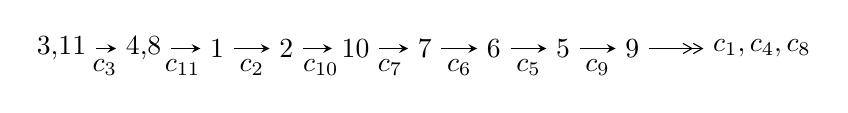
\begin{tikzpicture}[x=25pt, y=7pt]
	% node
	\node (A0) at (-1/8, 0) {3,11};
	\node (A1) at (17/16, 0) {4,8};
	\node (A2) at (17/8, 0) {1};
	\node (A3) at (25/8, 0) {2};
	\node (A4) at (33/8, 0) {10};
	\node (A5) at (41/8, 0) {7};
	\node (A6) at (49/8, 0) {6};
	\node (A7) at (57/8, 0) {5};
	\node (A8) at (65/8, 0) {9};
	\node (C1) at (1/2, -1) {$c_{3}$};
	\node (C2) at (13/8, -1) {$c_{11}$};
	\node (C3) at (21/8, -1) {$c_{2}$};
	\node (C4) at (29/8, -1) {$c_{10}$};
	\node (C5) at (37/8, -1) {$c_{7}$};
	\node (C6) at (45/8, -1) {$c_{6}$};
	\node (C7) at (53/8, -1) {$c_{5}$};
	\node (C8) at (61/8, -1) {$c_{9}$};
	\node (A9) at (10, 0) {$c_{1},c_{4},c_{8}$};

	% edge
	\draw[->,>=stealth]	
	(A0) edge (A1) (A1) edge (A2) (A2) edge (A3) (A3) edge (A4) (A4) edge (A5) (A5) edge (A6) (A6) edge (A7) (A7) edge (A8) ;
	\draw[->>,>={angle 60}]	
	(A8) edge (A9);
\end{tikzpicture} \\ 

\end{tabular} \\

\footnotetext{
The image of knot diagram is generated by the software ``\textbf{Draw programme}" developed by Andrew Bartholomew(\url{http://www.layer8.co.uk/maths/draw/index.htm\#Running-draw}), where we modified some parts for our purpose(\url{https://github.com/CATsTAILs/LinksPainter}).
}\phantom \\ \newline 
\centering \textbf{Ideals for irreducible components\footnotemark of $X_{\text{par}}$} 
 
\begin{align*}
I^u_{1}&=\langle 
-74 u^9+28 u^8+589 u^7-208 u^6-1099 u^5+580 u^4-535 u^3-218 u^2+439 b-447 u+41,\\
\phantom{I^u_{1}}&\phantom{= \langle  }-90 u^9-49 u^8+835 u^7+364 u^6-2357 u^5-576 u^4+1485 u^3-277 u^2+439 a+453 u+38,\\
\phantom{I^u_{1}}&\phantom{= \langle  }u^{10}+u^9-8 u^8-8 u^7+16 u^6+16 u^5+3 u^4-2 u^3+2 u+1\rangle \\
I^u_{2}&=\langle 
- u^6+u^5+3 u^4-2 u^3-2 u^2+b+u,\;u^4- u^3-3 u^2+a+2 u+2,\;u^7- u^6-4 u^5+3 u^4+5 u^3-2 u^2-2 u-1\rangle \\
I^u_{3}&=\langle 
-2 u^3+5 u^2+b+2 u-12,\;4 u^3-11 u^2+7 a-2 u+23,\;u^4- u^3-4 u^2+4 u+7\rangle \\
\\
\end{align*}
\raggedright * 3 irreducible components of $\dim_{\mathbb{C}}=0$, with total 21 representations.\\
\footnotetext{All coefficients of polynomials are rational numbers. But the coefficients are sometimes approximated in decimal forms when there is not enough margin.}
\newpage
\renewcommand{\arraystretch}{1}
\centering \section*{I. $I^u_{1}= \langle -74 u^9+28 u^8+\cdots+439 b+41,\;-90 u^9-49 u^8+\cdots+439 a+38,\;u^{10}+u^9+\cdots+2 u+1 \rangle$}
\flushleft \textbf{(i) Arc colorings}\\
\begin{tabular}{m{7pt} m{180pt} m{7pt} m{180pt} }
\flushright $a_{3}=$&$\begin{pmatrix}1\\0\end{pmatrix}$ \\
\flushright $a_{11}=$&$\begin{pmatrix}0\\u\end{pmatrix}$ \\
\flushright $a_{4}=$&$\begin{pmatrix}1\\- u^2\end{pmatrix}$ \\
\flushright $a_{8}=$&$\begin{pmatrix}0.205011 u^{9}+0.111617 u^{8}+\cdots-1.03189 u-0.0865604\\0.168565 u^{9}-0.0637813 u^{8}+\cdots+1.01822 u-0.0933941\end{pmatrix}$ \\
\flushright $a_{1}=$&$\begin{pmatrix}-0.931663 u^{9}-0.296128 u^{8}+\cdots-1.34396 u-0.362187\\0.558087 u^{9}+0.248292 u^{8}+\cdots+1.35763 u+0.542141\end{pmatrix}$ \\
\flushright $a_{2}=$&$\begin{pmatrix}-1.39180 u^{9}-0.635535 u^{8}+\cdots-1.96128 u-1.32346\\1.29841 u^{9}+0.373576 u^{8}+\cdots+1.46469 u+2.11845\end{pmatrix}$ \\
\flushright $a_{10}=$&$\begin{pmatrix}- u\\u\end{pmatrix}$ \\
\flushright $a_{7}=$&$\begin{pmatrix}0.275626 u^{9}+0.138952 u^{8}+\cdots-0.753986 u+0.239180\\0.0979499 u^{9}-0.0911162 u^{8}+\cdots+0.740319 u-0.419134\end{pmatrix}$ \\
\flushright $a_{6}=$&$\begin{pmatrix}0.373576 u^{9}+0.0478360 u^{8}+\cdots-0.0136674 u-0.179954\\0.0979499 u^{9}-0.0911162 u^{8}+\cdots+0.740319 u-0.419134\end{pmatrix}$ \\
\flushright $a_{5}=$&$\begin{pmatrix}-0.0933941 u^{9}-0.261959 u^{8}+\cdots-0.496583 u-1.20501\\-0.232346 u^{9}+0.00683371 u^{8}+\cdots-0.430524 u-0.168565\end{pmatrix}$ \\
\flushright $a_{9}=$&$\begin{pmatrix}0.205011 u^{9}+0.111617 u^{8}+\cdots-0.0318907 u-0.0865604\\0.168565 u^{9}-0.0637813 u^{8}+\cdots+1.01822 u-0.0933941\end{pmatrix}$\\ \flushright $a_{9}=$&$\begin{pmatrix}0.205011 u^{9}+0.111617 u^{8}+\cdots-0.0318907 u-0.0865604\\0.168565 u^{9}-0.0637813 u^{8}+\cdots+1.01822 u-0.0933941\end{pmatrix}$\\&\end{tabular}
\flushleft \textbf{(ii) Obstruction class $= -1$}\\~\\
\flushleft \textbf{(iii) Cusp Shapes $= -\frac{1240}{439} u^9-\frac{480}{439} u^8+\frac{9846}{439} u^7+\frac{3503}{439} u^6-\frac{18914}{439} u^5-\frac{5302}{439} u^4-\frac{7197}{439} u^3+\frac{1354}{439} u^2-\frac{490}{439} u-\frac{452}{439}$}\\~\\
\newpage\renewcommand{\arraystretch}{1}
\flushleft \textbf{(iv) u-Polynomials at the component}\newline \\
\begin{tabular}{m{50pt}|m{274pt}}
Crossings & \hspace{64pt}u-Polynomials at each crossing \\
\hline $$\begin{aligned}c_{1},c_{5}\end{aligned}$$&$\begin{aligned}
&u^{10}-6 u^9+\cdots-10 u+4
\end{aligned}$\\
\hline $$\begin{aligned}c_{2}\end{aligned}$$&$\begin{aligned}
&u^{10}+2 u^9+\cdots+20 u+16
\end{aligned}$\\
\hline $$\begin{aligned}c_{3},c_{4},c_{8}\\c_{10}\end{aligned}$$&$\begin{aligned}
&u^{10}+u^9-8 u^8-8 u^7+16 u^6+16 u^5+3 u^4-2 u^3+2 u+1
\end{aligned}$\\
\hline $$\begin{aligned}c_{6}\end{aligned}$$&$\begin{aligned}
&u^{10}+12 u^9+\cdots+1072 u+712
\end{aligned}$\\
\hline $$\begin{aligned}c_{7},c_{9}\end{aligned}$$&$\begin{aligned}
&u^{10}+2 u^9+\cdots-12 u+1
\end{aligned}$\\
\hline $$\begin{aligned}c_{11}\end{aligned}$$&$\begin{aligned}
&u^{10}+5 u^9+12 u^8+15 u^7+10 u^6+4 u^5+6 u^4+8 u^3+5 u^2+3 u+2
\end{aligned}$\\
\hline
\end{tabular}\\~\\
\newpage\renewcommand{\arraystretch}{1}
\flushleft \textbf{(v) Riley Polynomials at the component}\newline \\
\begin{tabular}{m{50pt}|m{274pt}}
Crossings & \hspace{64pt}Riley Polynomials at each crossing \\
\hline $$\begin{aligned}c_{1},c_{5}\end{aligned}$$&$\begin{aligned}
&y^{10}+2 y^9+\cdots+20 y+16
\end{aligned}$\\
\hline $$\begin{aligned}c_{2}\end{aligned}$$&$\begin{aligned}
&y^{10}+38 y^9+\cdots+3216 y+256
\end{aligned}$\\
\hline $$\begin{aligned}c_{3},c_{4},c_{8}\\c_{10}\end{aligned}$$&$\begin{aligned}
&y^{10}-17 y^9+\cdots-4 y+1
\end{aligned}$\\
\hline $$\begin{aligned}c_{6}\end{aligned}$$&$\begin{aligned}
&y^{10}+68 y^9+\cdots+2222848 y+506944
\end{aligned}$\\
\hline $$\begin{aligned}c_{7},c_{9}\end{aligned}$$&$\begin{aligned}
&y^{10}+46 y^9+\cdots-38 y+1
\end{aligned}$\\
\hline $$\begin{aligned}c_{11}\end{aligned}$$&$\begin{aligned}
&y^{10}- y^9+14 y^8-13 y^7+54 y^6-42 y^5+30 y^4+12 y^3+y^2+11 y+4
\end{aligned}$\\
\hline
\end{tabular}\\~\\
\newpage\flushleft \textbf{(vi) Complex Volumes and Cusp Shapes}
$$\begin{array}{c|c|c}  
\text{Solutions to }I^u_{1}& \I (\text{vol} + \sqrt{-1}CS) & \text{Cusp shape}\\
 \hline 
\begin{aligned}
u &= -0.303786 + 0.554609 I \\
a &= -1.19659 - 1.04112 I \\
b &= -0.210597 - 0.072758 I\end{aligned}
 & -1.58196 + 1.29510 I & -1.93721 + 1.18186 I \\ \hline\begin{aligned}
u &= -0.303786 - 0.554609 I \\
a &= -1.19659 + 1.04112 I \\
b &= -0.210597 + 0.072758 I\end{aligned}
 & -1.58196 - 1.29510 I & -1.93721 - 1.18186 I \\ \hline\begin{aligned}
u &= -0.595593 + 0.161209 I \\
a &= \phantom{-}1.251620 - 0.570638 I \\
b &= -0.897475 + 0.589151 I\end{aligned}
 & -0.62036 + 3.20996 I & \phantom{-}3.63110 - 5.43743 I \\ \hline\begin{aligned}
u &= -0.595593 - 0.161209 I \\
a &= \phantom{-}1.251620 + 0.570638 I \\
b &= -0.897475 - 0.589151 I\end{aligned}
 & -0.62036 - 3.20996 I & \phantom{-}3.63110 + 5.43743 I \\ \hline\begin{aligned}
u &= \phantom{-}0.470796 + 0.374659 I \\
a &= -0.742938 - 0.762785 I \\
b &= \phantom{-}0.262089 + 0.698748 I\end{aligned}
 & \phantom{-}1.01700 + 1.01665 I & \phantom{-}4.69191 - 3.41900 I \\ \hline\begin{aligned}
u &= \phantom{-}0.470796 - 0.374659 I \\
a &= -0.742938 + 0.762785 I \\
b &= \phantom{-}0.262089 - 0.698748 I\end{aligned}
 & \phantom{-}1.01700 - 1.01665 I & \phantom{-}4.69191 + 3.41900 I \\ \hline\begin{aligned}
u &= \phantom{-}2.01532 + 0.15224 I \\
a &= \phantom{-}0.624248 + 0.501185 I \\
b &= -0.19806 - 2.25477 I\end{aligned}
 & -19.7069 + 0.3487 I & \phantom{-}4.25811 + 0.03534 I \\ \hline\begin{aligned}
u &= \phantom{-}2.01532 - 0.15224 I \\
a &= \phantom{-}0.624248 - 0.501185 I \\
b &= -0.19806 + 2.25477 I\end{aligned}
 & -19.7069 - 0.3487 I & \phantom{-}4.25811 - 0.03534 I \\ \hline\begin{aligned}
u &= -2.08674 + 0.29586 I \\
a &= -0.436339 - 0.622756 I \\
b &= \phantom{-}0.54405 + 2.41435 I\end{aligned}
 & -19.4087 - 8.7708 I & \phantom{-}4.35608 + 3.79545 I \\ \hline\begin{aligned}
u &= -2.08674 - 0.29586 I \\
a &= -0.436339 + 0.622756 I \\
b &= \phantom{-}0.54405 - 2.41435 I\end{aligned}
 & -19.4087 + 8.7708 I & \phantom{-}4.35608 - 3.79545 I\\
 \hline 
 \end{array}$$\newpage\newpage\renewcommand{\arraystretch}{1}
\centering \section*{II. $I^u_{2}= \langle - u^6+u^5+3 u^4-2 u^3-2 u^2+b+u,\;u^4- u^3-3 u^2+a+2 u+2,\;u^7- u^6-4 u^5+3 u^4+5 u^3-2 u^2-2 u-1 \rangle$}
\flushleft \textbf{(i) Arc colorings}\\
\begin{tabular}{m{7pt} m{180pt} m{7pt} m{180pt} }
\flushright $a_{3}=$&$\begin{pmatrix}1\\0\end{pmatrix}$ \\
\flushright $a_{11}=$&$\begin{pmatrix}0\\u\end{pmatrix}$ \\
\flushright $a_{4}=$&$\begin{pmatrix}1\\- u^2\end{pmatrix}$ \\
\flushright $a_{8}=$&$\begin{pmatrix}- u^4+u^3+3 u^2-2 u-2\\u^6- u^5-3 u^4+2 u^3+2 u^2- u\end{pmatrix}$ \\
\flushright $a_{1}=$&$\begin{pmatrix}- u^6+u^5+3 u^4-2 u^3-3 u^2+u+2\\u^4- u^3-2 u^2+2 u\end{pmatrix}$ \\
\flushright $a_{2}=$&$\begin{pmatrix}- u^4+2 u^3+u^2-3 u+2\\- u^5+2 u^4+u^3-4 u^2+u+1\end{pmatrix}$ \\
\flushright $a_{10}=$&$\begin{pmatrix}- u\\u\end{pmatrix}$ \\
\flushright $a_{7}=$&$\begin{pmatrix}- u^4+3 u^2- u-2\\u^6- u^5-3 u^4+3 u^3+2 u^2-2 u\end{pmatrix}$ \\
\flushright $a_{6}=$&$\begin{pmatrix}u^6- u^5-4 u^4+3 u^3+5 u^2-3 u-2\\u^6- u^5-3 u^4+3 u^3+2 u^2-2 u\end{pmatrix}$ \\
\flushright $a_{5}=$&$\begin{pmatrix}- u^5+u^4+3 u^3-3 u^2-2 u+1\\u^5-3 u^3+2 u+1\end{pmatrix}$ \\
\flushright $a_{9}=$&$\begin{pmatrix}- u^4+u^3+3 u^2-3 u-2\\u^6- u^5-3 u^4+3 u^3+2 u^2- u\end{pmatrix}$\\ \flushright $a_{9}=$&$\begin{pmatrix}- u^4+u^3+3 u^2-3 u-2\\u^6- u^5-3 u^4+3 u^3+2 u^2- u\end{pmatrix}$\\&\end{tabular}
\flushleft \textbf{(ii) Obstruction class $= 1$}\\~\\
\flushleft \textbf{(iii) Cusp Shapes $= u^6+2 u^5-8 u^4-3 u^3+12 u^2$}\\~\\
\newpage\renewcommand{\arraystretch}{1}
\flushleft \textbf{(iv) u-Polynomials at the component}\newline \\
\begin{tabular}{m{50pt}|m{274pt}}
Crossings & \hspace{64pt}u-Polynomials at each crossing \\
\hline $$\begin{aligned}c_{1}\end{aligned}$$&$\begin{aligned}
&u^7- u^6+2 u^5-2 u^4+2 u^3-3 u^2+u-1
\end{aligned}$\\
\hline $$\begin{aligned}c_{2}\end{aligned}$$&$\begin{aligned}
&u^7+3 u^6+4 u^5-6 u^3-9 u^2-5 u-1
\end{aligned}$\\
\hline $$\begin{aligned}c_{3},c_{8}\end{aligned}$$&$\begin{aligned}
&u^7- u^6-4 u^5+3 u^4+5 u^3-2 u^2-2 u-1
\end{aligned}$\\
\hline $$\begin{aligned}c_{4},c_{10}\end{aligned}$$&$\begin{aligned}
&u^7+u^6-4 u^5-3 u^4+5 u^3+2 u^2-2 u+1
\end{aligned}$\\
\hline $$\begin{aligned}c_{5}\end{aligned}$$&$\begin{aligned}
&u^7+u^6+2 u^5+2 u^4+2 u^3+3 u^2+u+1
\end{aligned}$\\
\hline $$\begin{aligned}c_{6}\end{aligned}$$&$\begin{aligned}
&u^7+2 u^6-2 u^5-3 u^4-3 u^3+6 u^2- u+1
\end{aligned}$\\
\hline $$\begin{aligned}c_{7},c_{9}\end{aligned}$$&$\begin{aligned}
&u^7+2 u^6- u^5-3 u^4-2 u^3+u^2+2 u+1
\end{aligned}$\\
\hline $$\begin{aligned}c_{11}\end{aligned}$$&$\begin{aligned}
&u^7-2 u^6+u^5+2 u^4-3 u^3+u^2+2 u-1
\end{aligned}$\\
\hline
\end{tabular}\\~\\
\newpage\renewcommand{\arraystretch}{1}
\flushleft \textbf{(v) Riley Polynomials at the component}\newline \\
\begin{tabular}{m{50pt}|m{274pt}}
Crossings & \hspace{64pt}Riley Polynomials at each crossing \\
\hline $$\begin{aligned}c_{1},c_{5}\end{aligned}$$&$\begin{aligned}
&y^7+3 y^6+4 y^5-6 y^3-9 y^2-5 y-1
\end{aligned}$\\
\hline $$\begin{aligned}c_{2}\end{aligned}$$&$\begin{aligned}
&y^7- y^6+4 y^5-4 y^4+2 y^3-21 y^2+7 y-1
\end{aligned}$\\
\hline $$\begin{aligned}c_{3},c_{4},c_{8}\\c_{10}\end{aligned}$$&$\begin{aligned}
&y^7-9 y^6+32 y^5-57 y^4+51 y^3-18 y^2-1
\end{aligned}$\\
\hline $$\begin{aligned}c_{6}\end{aligned}$$&$\begin{aligned}
&y^7-8 y^6+10 y^5-23 y^4+45 y^3-24 y^2-11 y-1
\end{aligned}$\\
\hline $$\begin{aligned}c_{7},c_{9}\end{aligned}$$&$\begin{aligned}
&y^7-6 y^6+9 y^5-5 y^4+2 y^3-3 y^2+2 y-1
\end{aligned}$\\
\hline $$\begin{aligned}c_{11}\end{aligned}$$&$\begin{aligned}
&y^7-2 y^6+3 y^5-2 y^4+5 y^3-9 y^2+6 y-1
\end{aligned}$\\
\hline
\end{tabular}\\~\\
\newpage\flushleft \textbf{(vi) Complex Volumes and Cusp Shapes}
$$\begin{array}{c|c|c}  
\text{Solutions to }I^u_{2}& \I (\text{vol} + \sqrt{-1}CS) & \text{Cusp shape}\\
 \hline 
\begin{aligned}
u &= \phantom{-}1.212610 + 0.314318 I \\
a &= -0.186986 + 0.922572 I \\
b &= -0.25287 - 1.43719 I\end{aligned}
 & \phantom{-}4.41567 + 1.74618 I & \phantom{-}3.81474 - 1.89982 I \\ \hline\begin{aligned}
u &= \phantom{-}1.212610 - 0.314318 I \\
a &= -0.186986 - 0.922572 I \\
b &= -0.25287 + 1.43719 I\end{aligned}
 & \phantom{-}4.41567 - 1.74618 I & \phantom{-}3.81474 + 1.89982 I \\ \hline\begin{aligned}
u &= -1.303070 + 0.139348 I \\
a &= \phantom{-}0.819449 + 0.558129 I \\
b &= -0.275124 - 0.778615 I\end{aligned}
 & \phantom{-}2.10492 - 4.17967 I & \phantom{-}2.47305 + 4.17814 I \\ \hline\begin{aligned}
u &= -1.303070 - 0.139348 I \\
a &= \phantom{-}0.819449 - 0.558129 I \\
b &= -0.275124 + 0.778615 I\end{aligned}
 & \phantom{-}2.10492 + 4.17967 I & \phantom{-}2.47305 - 4.17814 I \\ \hline\begin{aligned}
u &= -0.278087 + 0.369158 I \\
a &= -1.48979 - 1.34313 I \\
b &= \phantom{-}0.466038 - 0.754209 I\end{aligned}
 & -1.45284 + 2.44043 I & -0.66357 - 2.79895 I \\ \hline\begin{aligned}
u &= -0.278087 - 0.369158 I \\
a &= -1.48979 + 1.34313 I \\
b &= \phantom{-}0.466038 + 0.754209 I\end{aligned}
 & -1.45284 - 2.44043 I & -0.66357 + 2.79895 I \\ \hline\begin{aligned}
u &= \phantom{-}1.73710\phantom{ +0.000000I} \\
a &= -0.285336\phantom{ +0.000000I} \\
b &= -0.876095\phantom{ +0.000000I}\end{aligned}
 & \phantom{-}6.31383\phantom{ +0.000000I} & \phantom{-}6.75150\phantom{ +0.000000I}\\
 \hline 
 \end{array}$$\newpage\newpage\renewcommand{\arraystretch}{1}
\centering \section*{III. $I^u_{3}= \langle -2 u^3+5 u^2+b+2 u-12,\;4 u^3-11 u^2+7 a-2 u+23,\;u^4- u^3-4 u^2+4 u+7 \rangle$}
\flushleft \textbf{(i) Arc colorings}\\
\begin{tabular}{m{7pt} m{180pt} m{7pt} m{180pt} }
\flushright $a_{3}=$&$\begin{pmatrix}1\\0\end{pmatrix}$ \\
\flushright $a_{11}=$&$\begin{pmatrix}0\\u\end{pmatrix}$ \\
\flushright $a_{4}=$&$\begin{pmatrix}1\\- u^2\end{pmatrix}$ \\
\flushright $a_{8}=$&$\begin{pmatrix}-\frac{4}{7} u^3+\frac{11}{7} u^2+\frac{2}{7} u-\frac{23}{7}\\2 u^3-5 u^2-2 u+12\end{pmatrix}$ \\
\flushright $a_{1}=$&$\begin{pmatrix}-\frac{5}{7} u^3+\frac{12}{7} u^2+\frac{6}{7} u-\frac{27}{7}\\1\end{pmatrix}$ \\
\flushright $a_{2}=$&$\begin{pmatrix}\frac{5}{7} u^3-\frac{12}{7} u^2-\frac{6}{7} u+\frac{34}{7}\\-1\end{pmatrix}$ \\
\flushright $a_{10}=$&$\begin{pmatrix}- u\\u\end{pmatrix}$ \\
\flushright $a_{7}=$&$\begin{pmatrix}\frac{10}{7} u^3-\frac{24}{7} u^2-\frac{12}{7} u+\frac{75}{7}\\-2\end{pmatrix}$ \\
\flushright $a_{6}=$&$\begin{pmatrix}\frac{10}{7} u^3-\frac{24}{7} u^2-\frac{12}{7} u+\frac{61}{7}\\-2\end{pmatrix}$ \\
\flushright $a_{5}=$&$\begin{pmatrix}\frac{15}{7} u^3-\frac{36}{7} u^2-\frac{18}{7} u+\frac{95}{7}\\-3\end{pmatrix}$ \\
\flushright $a_{9}=$&$\begin{pmatrix}\frac{3}{7} u^3-\frac{3}{7} u^2-\frac{12}{7} u+\frac{12}{7}\\u^3-2 u^2+u+5\end{pmatrix}$\\ \flushright $a_{9}=$&$\begin{pmatrix}\frac{3}{7} u^3-\frac{3}{7} u^2-\frac{12}{7} u+\frac{12}{7}\\u^3-2 u^2+u+5\end{pmatrix}$\\&\end{tabular}
\flushleft \textbf{(ii) Obstruction class $= -1$}\\~\\
\flushleft \textbf{(iii) Cusp Shapes $= -4 u^3+8 u^2+4 u-10$}\\~\\
\newpage\renewcommand{\arraystretch}{1}
\flushleft \textbf{(iv) u-Polynomials at the component}\newline \\
\begin{tabular}{m{50pt}|m{274pt}}
Crossings & \hspace{64pt}u-Polynomials at each crossing \\
\hline $$\begin{aligned}c_{1},c_{5}\end{aligned}$$&$\begin{aligned}
&(u+1)^4
\end{aligned}$\\
\hline $$\begin{aligned}c_{2}\end{aligned}$$&$\begin{aligned}
&(u-1)^4
\end{aligned}$\\
\hline $$\begin{aligned}c_{3},c_{4},c_{8}\\c_{10}\end{aligned}$$&$\begin{aligned}
&u^4- u^3-4 u^2+4 u+7
\end{aligned}$\\
\hline $$\begin{aligned}c_{6}\end{aligned}$$&$\begin{aligned}
&(u+2)^4
\end{aligned}$\\
\hline $$\begin{aligned}c_{7},c_{9}\end{aligned}$$&$\begin{aligned}
&u^4-3 u^3+2 u^2+6 u+13
\end{aligned}$\\
\hline $$\begin{aligned}c_{11}\end{aligned}$$&$\begin{aligned}
&(u^2- u+1)^2
\end{aligned}$\\
\hline
\end{tabular}\\~\\
\newpage\renewcommand{\arraystretch}{1}
\flushleft \textbf{(v) Riley Polynomials at the component}\newline \\
\begin{tabular}{m{50pt}|m{274pt}}
Crossings & \hspace{64pt}Riley Polynomials at each crossing \\
\hline $$\begin{aligned}c_{1},c_{2},c_{5}\end{aligned}$$&$\begin{aligned}
&(y-1)^4
\end{aligned}$\\
\hline $$\begin{aligned}c_{3},c_{4},c_{8}\\c_{10}\end{aligned}$$&$\begin{aligned}
&y^4-9 y^3+38 y^2-72 y+49
\end{aligned}$\\
\hline $$\begin{aligned}c_{6}\end{aligned}$$&$\begin{aligned}
&(y-4)^4
\end{aligned}$\\
\hline $$\begin{aligned}c_{7},c_{9}\end{aligned}$$&$\begin{aligned}
&y^4-5 y^3+66 y^2+16 y+169
\end{aligned}$\\
\hline $$\begin{aligned}c_{11}\end{aligned}$$&$\begin{aligned}
&(y^2+y+1)^2
\end{aligned}$\\
\hline
\end{tabular}\\~\\
\newpage\flushleft \textbf{(vi) Complex Volumes and Cusp Shapes}
$$\begin{array}{c|c|c}  
\text{Solutions to }I^u_{3}& \I (\text{vol} + \sqrt{-1}CS) & \text{Cusp shape}\\
 \hline 
\begin{aligned}
u &= -1.328780 + 0.090174 I \\
a &= \phantom{-}0.418587 - 0.623340 I \\
b &= \phantom{-}1.24248 + 1.97169 I\end{aligned}
 & \phantom{-}6.57974 + 2.02988 I & \phantom{-}8.00000 - 3.46410 I \\ \hline\begin{aligned}
u &= -1.328780 - 0.090174 I \\
a &= \phantom{-}0.418587 + 0.623340 I \\
b &= \phantom{-}1.24248 - 1.97169 I\end{aligned}
 & \phantom{-}6.57974 - 2.02988 I & \phantom{-}8.00000 + 3.46410 I \\ \hline\begin{aligned}
u &= \phantom{-}1.82878 + 0.77585 I \\
a &= -0.061444 + 0.499622 I \\
b &= \phantom{-}0.257518 - 1.105670 I\end{aligned}
 & \phantom{-}6.57974 + 2.02988 I & \phantom{-}8.00000 - 3.46410 I \\ \hline\begin{aligned}
u &= \phantom{-}1.82878 - 0.77585 I \\
a &= -0.061444 - 0.499622 I \\
b &= \phantom{-}0.257518 + 1.105670 I\end{aligned}
 & \phantom{-}6.57974 - 2.02988 I & \phantom{-}8.00000 + 3.46410 I\\
 \hline 
 \end{array}$$\newpage
\newpage\renewcommand{\arraystretch}{1}
\centering \section*{ IV. u-Polynomials}
\begin{tabular}{m{50pt}|m{274pt}}
Crossings & \hspace{64pt}u-Polynomials at each crossing \\
\hline $$\begin{aligned}c_{1}\end{aligned}$$&$\begin{aligned}
&(u+1)^4(u^7- u^6+2 u^5-2 u^4+2 u^3-3 u^2+u-1)\\
&\cdot(u^{10}-6 u^9+\cdots-10 u+4)
\end{aligned}$\\
\hline $$\begin{aligned}c_{2}\end{aligned}$$&$\begin{aligned}
&(u-1)^4(u^7+3 u^6+4 u^5-6 u^3-9 u^2-5 u-1)\\
&\cdot(u^{10}+2 u^9+\cdots+20 u+16)
\end{aligned}$\\
\hline $$\begin{aligned}c_{3},c_{8}\end{aligned}$$&$\begin{aligned}
&(u^4- u^3-4 u^2+4 u+7)(u^7- u^6-4 u^5+3 u^4+5 u^3-2 u^2-2 u-1)\\
&\cdot(u^{10}+u^9-8 u^8-8 u^7+16 u^6+16 u^5+3 u^4-2 u^3+2 u+1)
\end{aligned}$\\
\hline $$\begin{aligned}c_{4},c_{10}\end{aligned}$$&$\begin{aligned}
&(u^4- u^3-4 u^2+4 u+7)(u^7+u^6-4 u^5-3 u^4+5 u^3+2 u^2-2 u+1)\\
&\cdot(u^{10}+u^9-8 u^8-8 u^7+16 u^6+16 u^5+3 u^4-2 u^3+2 u+1)
\end{aligned}$\\
\hline $$\begin{aligned}c_{5}\end{aligned}$$&$\begin{aligned}
&(u+1)^4(u^7+u^6+2 u^5+2 u^4+2 u^3+3 u^2+u+1)\\
&\cdot(u^{10}-6 u^9+\cdots-10 u+4)
\end{aligned}$\\
\hline $$\begin{aligned}c_{6}\end{aligned}$$&$\begin{aligned}
&(u+2)^4(u^7+2 u^6-2 u^5-3 u^4-3 u^3+6 u^2- u+1)\\
&\cdot(u^{10}+12 u^9+\cdots+1072 u+712)
\end{aligned}$\\
\hline $$\begin{aligned}c_{7},c_{9}\end{aligned}$$&$\begin{aligned}
&(u^4-3 u^3+2 u^2+6 u+13)(u^7+2 u^6+\cdots+2 u+1)\\
&\cdot(u^{10}+2 u^9+\cdots-12 u+1)
\end{aligned}$\\
\hline $$\begin{aligned}c_{11}\end{aligned}$$&$\begin{aligned}
&(u^2- u+1)^2(u^7-2 u^6+u^5+2 u^4-3 u^3+u^2+2 u-1)\\
&\cdot(u^{10}+5 u^9+12 u^8+15 u^7+10 u^6+4 u^5+6 u^4+8 u^3+5 u^2+3 u+2)
\end{aligned}$\\
\hline
\end{tabular}\newpage\renewcommand{\arraystretch}{1}
\centering \section*{ V. Riley Polynomials}
\begin{tabular}{m{50pt}|m{274pt}}
Crossings & \hspace{64pt}Riley Polynomials at each crossing \\
\hline $$\begin{aligned}c_{1},c_{5}\end{aligned}$$&$\begin{aligned}
&(y-1)^4(y^7+3 y^6+4 y^5-6 y^3-9 y^2-5 y-1)\\
&\cdot(y^{10}+2 y^9+\cdots+20 y+16)
\end{aligned}$\\
\hline $$\begin{aligned}c_{2}\end{aligned}$$&$\begin{aligned}
&(y-1)^4(y^7- y^6+4 y^5-4 y^4+2 y^3-21 y^2+7 y-1)\\
&\cdot(y^{10}+38 y^9+\cdots+3216 y+256)
\end{aligned}$\\
\hline $$\begin{aligned}c_{3},c_{4},c_{8}\\c_{10}\end{aligned}$$&$\begin{aligned}
&(y^4-9 y^3+38 y^2-72 y+49)(y^7-9 y^6+\cdots-18 y^2-1)\\
&\cdot(y^{10}-17 y^9+\cdots-4 y+1)
\end{aligned}$\\
\hline $$\begin{aligned}c_{6}\end{aligned}$$&$\begin{aligned}
&(y-4)^4(y^7-8 y^6+10 y^5-23 y^4+45 y^3-24 y^2-11 y-1)\\
&\cdot(y^{10}+68 y^9+\cdots+2222848 y+506944)
\end{aligned}$\\
\hline $$\begin{aligned}c_{7},c_{9}\end{aligned}$$&$\begin{aligned}
&(y^4-5 y^3+66 y^2+16 y+169)\\
&\cdot(y^7-6 y^6+\cdots+2 y-1)(y^{10}+46 y^9+\cdots-38 y+1)
\end{aligned}$\\
\hline $$\begin{aligned}c_{11}\end{aligned}$$&$\begin{aligned}
&(y^2+y+1)^2(y^7-2 y^6+3 y^5-2 y^4+5 y^3-9 y^2+6 y-1)\\
&\cdot(y^{10}- y^9+14 y^8-13 y^7+54 y^6-42 y^5+30 y^4+12 y^3+y^2+11 y+4)
\end{aligned}$\\
\hline
\end{tabular}
\vskip 2pc
\end{document}